\chapter{Электрические измерения}

% Системы единиц. Урезать. Оставить только таблицы в конце
%\vn О системах единиц в классической электродинамике

При измерении физической величины $x$ её числовое значение \fs{x} свидетельствует о том, сколько раз в $x$ содержится
некоторая единица измерения \ks{x}. Это означает, что
\be1
\fs{x}=\frac{x}{\ks{x}}.
\ee
Если, например, сила тока $I=10$~А, то $\fs{I}=10$, $\ks{I}=1$~А. Соотношение (\r1) можно записать в виде
\be2
x=\fs{x}\ks{x}.
\ee
При уменьшении единицы измерения в $\alpha$ раз
\[
\ks{x}\rightarrow\ks{X}=\frac{1}{\alpha}\ks{x},\qquad\fs{x}\rightarrow\fs{X}=\alpha\fs{x}.
\]
Сама физическая величина при этом не изменяется, поскольку
\be3
x=\fs{x}\ks{x}=\fs{X}\ks{X}.
\ee

Для каждой физической величины можно в принципе установить свою единицу, никак не связанную с единицами других величин.
Это приводит, однако, к тому, что в уравнениях, выражающих физические законы, появляется множество численных
коэффициентов. Уравнения становятся необозримыми, формулы~--- слишком сложными. Чтобы избежать этого, в физике уже давно
отказались от независимого выбора единиц всех физических величин и стали применять системы единиц, построенные по
определённому принципу, который состоит в следующем. Некоторые величины принимаются за базисные, т.е. такие, для которых
единицы устанавливаются произвольно. Так, например, в механике применяется система ($L$, $M$, $T$), в которой за базисные
величины принимаются длина $L$, масса $M$ и время $T$. Выбор базисных величин и их число произвольны. Это вопрос
соглашения. В международной системе СИ в качестве базисных величин приняты девять величин: длина, масса, время, сила
электрического тока, температура, сила света, количество вещества, плоский угол, телесный угол. Величины, не являющиеся
базисными, называются производными. Для производных величин единицы устанавливаются на основе формул, служащих их
определением.

Здесь возникает понятие размерности. Если, например, число базисных величин равно трём и за них приняты длина $L$, масса
$M$ и время $T$, то для размерности производной величины $y$ имеем
\be4
\dim y=L^p\cdot M^q\cdot T^r,
\ee
где $p$, $q$, $r$~--- постоянные числа. Формула (\r4) показывает, что если единицы длины, массы и времени уменьшить в
$\alpha$, $\beta$ и $\gamma$ раз, то единица производной величины $y$ уменьшится в $\alpha^p\beta^q\gamma^r$ раз, и,
следовательно, её числовое значение увеличится в такое же число раз. В этом и состоит смысл понятия размерности.
Заметим, что для безразмерной величины~$z$
\[
\dim z=1.
\]
На практике величины $p$, $q$, $r$ оказываются рациональными числами. Это обусловлено соответствующими определениями
физических величин.

Часто размерность физической величины отождествляют с её единицей в соответствующей системе единиц. Так, например,
говорят, что скорость имеет размерность $м/с$, а давление $Н/м^2$. В этом нет большой беды, хотя, строго говоря, это
неверно: размерность скорости~--- $LT^{-1}$, а давления~--- $ML^{-1}T^{-2}$.

Рассмотрим вопрос о системах единиц в электродинамике. Законы макроскопической электродинамики определяются её
фундаментальными аксиомами~--- уравнениями Максвелла, которые являются концентрированным обобщением экспериментальных
фактов из области электричества и магнетизма. Запишем уравнения Максвелла для вакуума в произвольной системе единиц:

\def\urtab#1#2#3{%
\vskip-1ex
\be#3
\begin{array}{ll}
\hbox to 0.5\textwidth{$\ds #1$\hfil}&\hbox to 0.25\textwidth{$\ds #2$\hfil}
\end{array}
\ee
\vskip-1ex
}

\urtab{\oint_S \vec{E}d\vec{S}=\alpha\int_V\rho\,dV,}{\divv\vec{E}=\alpha\rho,}{5}

\urtab{\oint_S\vec{B}d\vec{S}=0,}{\divv\vec{B}=0,}{6}

\urtab{\oint_L\vec{E}d\vec{l}=-\beta\int_S\frac{\d{\vec{B}}}{\d t}\,d\vec{S},}{\rot\vec{E}=-\beta\frac{\d\vec B}{\d t},}{7}

\urtab{\oint_L\vec{B}d\vec{l}=\gamma\int_S\vec{j}\,d\vec{S}+\delta\int_S\frac{\d{\vec{E}}}{\d t}\,d\vec{S},}
{\rot\vec{B}=\gamma\vec{j}+\delta\frac{\d\vec E}{\d t};}{8}

\be9
\vec{F}=\xi q\vec{E}+\eta q\vec{v}\times\vec{B},
\ee
\be10
d\vec{F}=\xi dq\vec{E}+\eta Id\vec{l}\times\vec{B}.
\ee
Здесь приняты стандартные обозначения. Уравнение (\r9) или (\r{10}) служит для определения силовых векторов $\vec{E}$ и
$\vec{B}$. Множество коэффициентов ($\alpha$, $\beta$, $\gamma$, $\delta$, $\xi$, $\eta$) свидетельствует о том, что для
каждой физической величины, входящей в систему уравнений (\r5)~--~(\r{10}), принята собственная единица измерения,
независимая от единиц других величин.

Напомним физический смысл уравнений Максвелла. Уравнение (\r5) показывает, что источником электрического поля $\vec{E}$
является электрический заряд. Из него можно получить закон Кулона:
\be11
\vec{F}_{12}=\alpha\frac{q_1q_2}{4\pi r^3_{12}}\vec{r}_{12}.
\ee
Уравнение (\r6) говорит о том, что в природе отсутствуют, насколько известно в настоящее время, магнитные заряды.
Уравнение (\r7)~--- это математическая формулировка закона электромагнитной индукции. Оно свидетельствует о том, что
изменяющееся магнитное поле порождает вихревое электрическое поле. Уравнение (\r8) показывает, что магнитное поле
$\vec{B}$~--- всегда вихревое (силовые линии замкнуты), и его источником являются не только движущиеся заряды, но и
переменное электрическое поле. Для постоянного магнитного поля с помощью (\r8) можно получить закон Био--Савара (см.
Приложение):
\be12
d\vec{B}=\frac{\gamma}{4\pi}\frac{I\,d\vec{l}\times\vec{r}}{r^3}.
\ee

С помощью уравнения
\[
\oint\vec{B}\cdot d\vec{l}=\gamma\int\vec{j}\cdot\vec{S}
%\rot\vec{B}=\gamma\vec{j}
\]
можно найти отнесённую к единице длины силу взаимодействия между двумя токами $I_1$ и $I_2$, текущими по двум бесконечно
длинным параллельным проводам:
\be13
\frac{dF}{dl}=\gamma\eta\frac{I_1I_2}{2\pi r}.
\ee

Рассмотрим электромагнитное поле в области, где нет источников, т.е. $\rho=0$ и $\vec{j}=0$. В силу (\r7) и (\r8) имеем
\[
\rot\,\rot\vec{E}=-\beta\frac{\d}{\d t}\rot\vec{B}=-\beta\delta\frac{\d^2\vec{E}}{\d t^2}
\]
или
\[
\grad\,\divv\vec{E}-\nabla^2\vec{E}=-\beta\delta\frac{\d^2\vec{E}}{\d t^2},
\]
т.е.
\be14
\nabla^2\vec{E}=\beta\delta\frac{\d^2\vec{E}}{\d t^2}.
\ee
Волновое уравнение (\r{14}) описывает распространение электромагнитных волн в вакууме. Скорость распространения волн
равна ${1}/{\sqrt{\beta\delta}}$. Измерения дают ${1}/\sqrt{\beta\delta}=c$, где $c$~--- скорость света в вакууме. Таким
образом, из опыта следует, что $\beta\delta=1/c^2$, где $c$~--- универсальная фундаментальная постоянная.

Запишем уравнения (\r5)~--~(\r9) в безразмерном виде. Для каждой физической величины $f$, входящей в эту систему, введём
следующие обозначения:
\be15
\fs{f}\equiv f',\quad\ks{f}\equiv f_0,\quad\text{т.е.}\quad f'=\frac{f}{f_0}\quad или\quad f=f'\.f_0.
\ee
Для единиц длины $l$ и времени $\tau$ имеем
\be16
\vec{r}=\vec{r}\,'\cdot l,\qquad t=t'\cdot\tau.
\ee

Подставляя (\r{15}) и (\r{16}) в систему (\r5)~--~(\r9) и опуская штрихи, находим

\def\urtab#1#2#3{%
\vskip-1ex
\be#3
\begin{array}{ll}
\hbox to 0.5\textwidth{$\ds #1$\hfil}&\hbox to 0.3\textwidth{$\ds #2$\hfil}
\end{array}
\ee
\vskip-1ex
}

\urtab{E_0l^2\oint_S \vec{E}d\vec{S}=\alpha\rho_0l^3\int_V\rho\,dV,}
{\frac{E_0}{l}\divv \vec{E}=\alpha\rho_0\rho,}{17}

\urtab{\oint_S\vec{B}d\vec{S}=0,}{\divv\vec{B}=0,}{18}

\urtab{E_0l\oint_L\vec{E}d\vec{l}=-\beta\frac{B_0}{\tau}l^2\int_S\frac{\d{\vec{B}}}{\d t}\,d\vec{S},}
{\frac{E_0}{l}\rot\vec{E}=-\frac{\beta B_0}{\tau}\frac{\d\vec B}{\d t},}{19}

%B_0l\oint_L\vec{B}d\vec{l}=
%\gamma j_0l^2\int_S\vec{j}\,d\vec{S}+\delta\frac{E_0l^2}{\tau}\int_S\frac{\d{\vec{E}}}{\d t}\,d\vec{S}&
%\frac{B_0}{l}\rot\vec{B}=\gamma j_0\vec{j}+\frac{\delta E_0}{\tau}\frac{\d\vec E}{\d t},&\num{20}\\


\be20
\begin{array}{ll}
\hbox to 0.4\textwidth{$\ds B_0l\oint_L\vec{B}d\vec{l}=
\gamma j_0l^2\int_S\vec{j}\,d\vec{S}+\delta\frac{E_0l^2}{\tau}\int_S\frac{\d{\vec{E}}}{\d t}\,d\vec{S},$\hss}&\\ [4ex]
&\ds\frac{B_0}{l}\rot\vec{B}=\gamma j_0\vec{j}+\frac{\delta E_0}{\tau}\frac{\d\vec E}{\d t},
\end{array}
\ee

\iffalse
\be17
E_0l^2\oint_S \vec{E}d\vec{S}=\alpha\rho_0l^3\int_V\rho\,dV
\qquad\frac{E_0}{l}\divv \vec{E}=\alpha\rho_0\rho,
\ee
\be18
\oint_S \vec{B}d\vec{S}=0
\qquad\divv \vec{B}=0,
\ee
\be19
E_0l\oint_L\vec{E}d\vec{l}=-\beta\frac{B_0}{\tau}l^2\int_S\frac{\d{\vec{B}}}{\d t}\,d\vec{S}
\qquad\frac{E_0}{l}\rot\vec{E}=-\frac{\beta B_0}{\tau}\frac{\d\vec B}{\d t},
\ee
\be20
B_0l\oint_L\vec{B}d\vec{l}=\gamma j_0l^2\int_S\vec{j}\,d\vec{S}+\delta\frac{E_0l^2}{\tau}\frac{\d{\vec{E}}}{\d t}\,d\vec{S}
\qquad\frac{B_0}{l}\rot\vec{B}=\gamma j_0\vec{j}+\frac{\delta E_0}{\tau}\frac{\d\vec E}{\d t},
\ee

\fi

\be21
F_0\vec{F}=\xi q_0qE_0\vec{E}+\eta q_0qv_0B_0\vec{v}\times\vec{B}.
\ee
Здесь $\ds v_0=\frac{l}{\tau}$, $j_0=\rho_0v_0$.

Из (\r{17})~--~(\r{21}) следует, что
\[
\dim\alpha=\dim\frac{E_0}{\rho_0l},
\]
\[
\dim\beta=\dim\frac{1}{v_0}\frac{E_0}{B_0},
\]
\[
\dim\gamma=\dim\frac{B_0}{j_0l},
\]
\[
\dim\frac{\delta}{\gamma}=\dim\frac{j_0\tau}{E_0}=\dim\frac{\rho_0v_0\tau}{E_0}=\dim\frac{\rho_0l}{E_0},
\]
\[
\dim\delta=\dim\frac{1}{v_0}\frac{B_0}{E_0},
\]
\[
\dim\frac{\xi}{\eta}=\dim v_0\frac{B_0}{E_0}.
\]
Отсюда можно видеть, что
\[
\dim\frac{\alpha\delta}{\gamma}=1,\qquad \dim\frac{\xi\beta}{\eta}=1,
\]
\[
\dim\delta\beta=\dim\frac{1}{v_0^2}.
\]
Последнее соответствует тому, что
\[
\delta\beta=\frac{1}{c^2}.
\]
При выборе базисных единиц естественно предположить, что
\be22
\frac{\alpha\delta}{\gamma}=1,\quad\frac{\xi\beta}{\eta}=1,\quad \delta\beta=\frac{1}{c^2}.
\ee
В таблице \r{tab1} показано, как в различных системах пользуются произволом, который дают соотношения (\r{22}). В
настоящее время принято считать, что $c=299\,792\,458$~м/с (точно). Это означает, что базисные единицы <<привязаны>> к
этой величине. Это, конечно, соглашение. Мы полагаем в лаборатории $c\cong3\.10^8$~м/с.

В общей физике в настоящее время используются в основном две системы единиц: гауссова система СГС (далее~--- система СГС)
и международная система СИ (далее~--- система СИ). Система СГС, в которой в качестве базисных величин приняты длина,
масса и время, разработана на основе законов механики Ньютона. Электрические и магнитные величины вводятся в ней как
производные механических. Построенные по такому принципу системы единиц называются абсолютными. В системе СГС
электрические величины измеряются в единицах СГСЭ, а магнитные~--- в единицах СГСМ.

В системе СИ к трём базисным механическим величинам~--- длине, времени и массе~--- в электродинамике добавлена
независимая чисто электрическая величина, имеющая собственную размерность. В качестве таковой выбрана сила
электрического тока, а её единицей выбран ампер. Единицей заряда при этом является ампер-секунда, называемая кулоном.

\begin{table}[!t]
\tab{1}{Некоторые системы единиц, используемые при изучении макроскопической электродинамики}{%
\def\vph{\vphantom{$\ds\frac{A}{B}$}}\def\pp#1{\hbox to 5mm{\hfil #1\hfil}}%
\bt{|l|c|c|c|c|c|c|c|c|c|}\hline
\vph&\pp{$\alpha$}&\pp{$\beta$}&\pp{$\gamma$}&\pp{$\delta$}&\pp{$\xi$}&\pp{$\eta$}&\pp{$\frac{\alpha\delta}{\gamma}$}&
\pp{$\frac{\xi\beta}{\eta}$}&\pp{$\delta\beta$}\\ \hline
\vph СГСЭ&$4\pi$&1&$\frac{4\pi}{c^2}$&$\frac{1}{c^2}$&1&1&1&1&$\frac{1}{c^2}$\\ \hline
\vph СГСМ&$4\pi c^2$&1&$4\pi$&$\frac{1}{c^2}$&1&1&1&1&$\frac{1}{c^2}$\\ \hline
\vph СГС&$4\pi$&$\frac{1}{c}$&$\frac{4\pi}{c}$&$\frac{1}{c}$&1&$\frac{1}{c}$&1&1&$\frac{1}{c^2}$\\ \hline
\vph СИ&$\frac{1}{\e_0}$&1&$\frac{1}{\e_0c^2}$&$\frac{1}{c^2}$&1&1&1&1&$\frac{1}{c^2}$\\ \hline
\vph МКС&1&1&$\frac{1}{c^2}$&$\frac{1}{c^2}$&1&1&1&1&$\frac{1}{c^2}$\\ \hline
\multicolumn{10}{|l|}{\vph \hskip 1cm $c=299\,792\,458$~м/с (точно);}\\
\multicolumn{10}{|l|}{\vph\hskip 1cm $\e_0=8,854\.10^{-12}$~Ф/м;~~~$\mu_0=\frac{1}{\e_0c^2}=4\pi\.10^{-7}$~Гн/м.}\\ \hline
\et
}
\vskip-2em
\end{table}

Эталон силы электрического тока устанавливается на основе формулы (\r{13}). В системе СИ $\gamma=\frac{1}{\e_0c^2}$,
$\eta=1$, поэтому
\be23
\D F=\frac{1}{\e_0c^2}\frac{I_1I_2}{2\pi r}\D l.
\ee
На основании международного соглашения принято по определению, что ампер~--- это единица силы тока, который, проходя по
двум параллельным прямолинейным проводникам бесконечной длины и исчезающе малого кругового сечения, расположенным на
расстоянии 1~м друг от друга в вакууме, вызывал бы между проводниками силу, равную $2\.10^{-7}$~Н на каждый метр длины.
Реализовать эту единицу можно несколькими способами, например, измеряя силу взаимодействия двух катушек с постоянным
током.

Полагая в (\r{23}) $I_1=I_2=1$~А, имеем
\[
2\.10^{-7}~Н=\frac{1}{\e_0c^2}\frac{1}{2\pi}~Н,
\]
т.е.
\[
\frac{1}{\e_0c^2}=4\pi\.10^{-7}~\text{ед. СИ}
\]
или
\[
\e_0=\frac{10^{7}}{4\pi c^2}\approx 8,85\.10^{-12}~\text{ед. СИ.}
\]

В системе СГС единиц формула (\r{13}) имеет вид
\be24
\D F=\frac{4\pi}{c^2}\frac{I_1I_2}{2\pi r}\D l.
\ee

Установим соотношение между единицами силы электрического тока в системе СГС и системе СИ. Полагая в (\r{23})
$I_1=I_2=1$~А, $r=\D l=1$~м, находим
\be25
\D F=2\.10^{-7}~Н.
\ee
Воспользуемся теперь для вычисления той же силы формулой (\r{24}). Полагая в этой формуле $I_1=I_2=I$, $r=\D l=100$~см,
находим
\be26
\D F=\frac{4\pi}{c^2}\frac{I^2}{2\pi}=\frac{2I^2}{c^2}~дин=\frac{2I^2}{c^2}10^{-5}~Н.
\ee
Приравнивая (\r{25}) и (\r{26}), имеем
\[
2\.10^{-7}=\frac{2I^2}{c^2}10^{-5},\qquad т.е.\qquad I=3\.10^9~\text{ед. СГС}.
\]
Это означает, что
\be27
10\ks{I}_{СИ}=c\ks{I}_{СГС},
\ee
где $c=3\.10^{10}$~см/с, $\ks{I}_{СИ}=1$~А. Соотношение (\r{27}) можно представить в виде
\[
\ks{I}_{СИ}=3\.10^9\ks{I}_{СГС}
\]
или
\be28
c=10\frac{\fs{I}_{СГС}}{\fs{I}_{СИ}}\left(\frac{см}{с}\right),
\ee
что может быть проверено экспериментально (см. работу \textnumero~3.1.1).

В силу (\r{27}) для электрического заряда имеем
\[
\ks{q}_{СИ}=3\.10^9\ks{q}_{СГС}.
\]
Установим соотношение между единицами разности потенциалов в системе СГС и системе СИ. Воспользуемся для этого формулой
для отсчитываемого от бесконечно удалённой точки потенциала точечного заряда:
\[
\phi=\frac{q}{r}\quad (СГС),\qquad\qquad
\phi=\frac{1}{4\pi\e_0}\frac{q}{r}\quad (СИ).
\]
Пусть $q=1$~ед. СГС, а $r=1$~см, тогда $\phi=1~ед.~СГС\equiv\ks{\phi}_{СГС}$. Вычислим этот же потенциал в системе СИ:
\[
\phi=\frac{9\.10^9}{3\.10^9\cdot10^{-2}}=300~В.
\]
Это означает, что для единиц разности потенциалов имеем
\be29
\ks{U}_{СГС}=300\ks{U}_{СИ}.
\ee
Соотношение (\r{29}) может быть также проверено экспериментально, например, с помощью абсолютного вольтметра (см. работу
\textnumero~3.1.2).

Подобным образом устанавливаются соотношения между единицами других физических систем, величин (см. таблицу~\r{tab2}).
Основные формулы в системах СИ и СГС представлены в таблице~\r{tab3}.

\newpage

\tab{2}{Перевод числовых значений физических величин из~системы СИ в~систему СГС}{%
%\def\vs{\vphantom{$\ds\frac{A}{B}$}}%
\let\vs=\tabstrut
\def\bbx{\raggedright\baselineskip=9pt}%
\def\pbl#1#2{\parbox{#1}{\bbx #2}}%
\def\vr{\vbox to 3pt{}}%
\def\pb#1{$\vcenter{\vr\hbox{\pbl{30mm}{#1\hfill}}\vr}$}%
\bt{|l|c|c|c|}\hline
\vs Наименование&Обозн.&СИ&СГС\\ \hline
\vs Длина&$l$&1 м (метр)&$10^2$~см\\ \hline
\vs Масса&$m$&1 кг (килограмм)&$10^3$ г\\ \hline
\vs Время&$t$&1 с (секунда)&1 с\\ \hline
\vs Работа, энергия&$A$, $W$&1 Дж (джоуль)&$10^7$ эрг\\ \hline
\vs Мощность&$N$&1 Вт (ватт)&$10^7~\frac{эрг}{с\mathstrut}$\\ \hline
\vs Давление&$P$&1 Па (паскаль)&$10~\frac{дин}{см^2\mathstrut}$\\ \hline
\vs \pb{Сила электри-\\ческого тока}&$I$&1 А (ампер)&$3\.10^9$\\ \hline
\vs Электр. заряд&$q$&1 Кл (кулон)&$3\.10^9$\\ \hline
\vs Поляризация&$\vec{P}$&$1~\frac{Кл}{м^2}$&$3\.10^5$\\ \hline
\vs \pb{Электрическая индукция}&$\vec{D}$&$1~\frac{Кл}{м^2}$&$12\pi\.10^5$\\ \hline
\vs Электр. ёмкость&$C$&1 Ф (фарад)&$9\.10^{11}$ см\\ \hline
\vs \pb{Электрическое сопротивление}&$R$&1 Ом (ом)&$\frac{1}{9\.10^{11}}~\frac{с}{см\mathstrut}$\\ \hline
\vs \pb{Удельное сопротивление}&$\rho$&1 Ом\.м&$\frac{1}{9\.10^{9}\mathstrut}~с$\\ \hline
\vs \pb{Электрическая проводимость}&$\Lambda=\frac{1}{R}$&1 См (сименс)&$9\.10^{11}~\frac{см}{с\mathstrut}$\\ \hline
\vs \pb{Удельная проводимость}&$\sigma$&$1~\frac{См}{м}$&$9\.10^9~с^{-1}$\\ \hline
\vs Магнитный поток&$\Phi$&1 Вб (вебер)&$10^8$ Мкс\\ \hline
\vs \pb{Магнитная индукция}&$\vec{B}$&1 Тл (тесла)&$10^4$ Гс\\ \hline
\vs \pb{Напряжённость магнитного поля}&$\vec{H}$&$1~\frac{А}{м}$&$4\pi\cdot10^{-3}$ Э\\ \hline
\vs Намагниченность&$\vec{M}$&$1~\frac{А}{м}$&$\frac{1}{4\pi}\cdot 10^4$ Гс\\ \hline
\vs Индуктивность&$L$&1 Гн (генри)&$10^9$ см\\ \hline
\vs \pb{Электрический потенциал}&$\phi$&$1~В$ (вольт)&$\frac{1}{300}$\\ \hline
\vs \pb{Напряжённость электр. поля}&$\vec{E}$&$1~\frac{В}{м}$&$\frac{1}{3}\cdot 10^{-4}$\\ \hline
\et
}

\newpage

%\ftab{
\tab{3}{Основные формулы в СИ и СГС}{\small%
\let\vs=\tabstrut
\def\bbx{\raggedright\baselineskip=10pt}%
\def\pbl#1#2{\parbox{#1}{\bbx #2}}%
\def\vr{\vbox to 2pt{}}%
\def\pb#1{\vs$\vcenter{\vr\hbox{\pbl{38mm}{#1\hfill}}\vr}$}%
\bt{l|c|c}\hline
\vs Наименование&СИ&СГС\\ \hline
\pb{Уравнения Максвелла}&$\divv\vec{D}=\rho$&$\divv\vec{D}=4\pi\rho$\\
\pb{в дифференциальной}&$\divv\vec{B}=0$&$\divv\vec{B}=0$\\
\pb{форме}&$\rot\vec{E}=-\frac{\d\vec{B}}{\d t}$&$\rot\vec{E}=-\frac{1}{c}\frac{\d\vec{B}}{\d t}$\\
\pb{}&$\rot\vec{H}=\vec{j}+\frac{\d\vec{D}}{\d t}$&$\rot\vec{H}=\frac{4\pi}{c}\vec{j}+\frac{1}{c}\frac{\d\vec{D}}{\d t}$\\
\pb{Электрическая индукция}&$\vec{D}=\e_0\vec{E}+\vec{P}$&$\vec{D}=\vec{E}+4\pi\vec{P}$\\
\pb{Напряжённость магнитного поля}&$\vec{H}=\frac{1}{\mu_0}\vec{B}-\vec{M}$&$\vec{H}=\vec{B}-4\pi\vec{M}$\\
\\
\pb{Материальные}&$\vec{P}=\alpha\e_0\vec{E}$&$\vec{P}=\alpha\vec{E}$\\
\pb{уравнения}&$\vec{D}=\e\e_0\vec{E}$&$\vec{D}=\e\vec{E}$\\
%\pb{Связь между $\vec{D}$ и $\vec{E}$ в~вакууме}&$\vec{D}=\e_0\vec{E}$&$\vec{D}=\vec{E}$\\
&$\vec{M}=\kappa\vec{H}$&$\vec{M}=\kappa\vec{H}$\\
&$\vec{B}=\mu\mu_0\vec{H}$&$\vec{B}=\mu\vec{H}$\\
\pb{}&$\vec{j}=\sigma\vec{E}$&$\vec{j}=\sigma\vec{E}$\\
\\
%\pb{Связь между $\vec{B}$ и $\vec{H}$ в~вакууме}&$\vec{B}=\mu_0\vec{H}$&$\vec{B}=\vec{H}$\\
\pb{Уравнения Максвелла}&$\oint\limits_{S}\v{D}\,d\v{S}=\int_{V}\rho\,dV$&
$\oint\limits_{S}\v{D}\,d\v{S}=4\pi\int_{V}\rho\,dV$\\
\pb{в интегральной форме}&$\oint\limits_{S}\v{B}\,d\v{S}=0$&$\oint\limits_{S}\v{B}\,d\v{S}=0$\\
\pb{}&$\oint\limits_{L}\v{E}\,d\v{l}=-\int_{S}\frac{\d\vec{B}}{\d t}\,d\vec{S}$&
$\oint\limits_{L}\v{E}\,d\v{l}=-\frac{1}{c}\int_{S}\frac{\d\vec{B}}{\d t}\,d\vec{S}$\\
\pb{}&$\oint\limits_{L}\v{H}\,d\v{l}=$~~~~~~~~~~&$\oint\limits_{L}\v{H}\,d\v{l}=$~~~~~~~~~~\\
\pb{}&$=\int_{S}\vec{j}\,d\vec{S}+\int_{S}\frac{\d\vec{D}}{\d t}\,d\vec{S}$&
$=\frac{4\pi}{c}\int_{S}\vec{j}\,d\vec{S}+\frac{1}{c}\int_{S}\frac{\d\vec{D}}{\d t}\,d\vec{S}$\\
\pb{Сила Лоренца}&$\vec{F}=q\v{E}+\vp{\vec{v}}{\vec{B}}$&
$\ds\vec{F}=q\v{E}+\frac{q\mathstrut}{c\mathstrut}\vp{\vec{v}}{\vec{B}}$\\
\pb{Закон Кулона}&$\ds \v{F}=\frac{1}{4\pi\e_0}\frac{q_1q_2}{\e r^3}\v{r}$&$\ds\v{F}=\frac{q_1q_2}{\e r^3}\v{r}$\\[2ex]
\pb{Закон Био--Савара}&$\ds d\vec{H}=\frac{I}{4\pi}\frac{\vp{d\vec{l}}{\vec{r}}}{r^3}$&
$\ds d\vec{H}=\frac{I}{c}\frac{\vp{d\vec{l}}{\vec{r}}}{r^3}$\\[2ex]
\pb{Закон Ампера}&$d\vec{F}=I\vp{d\vec{l}}{\vec{B}}$&$d\vec{F}=\frac{I}{c}\vp{d\vec{l}}{\vec{B}}$\\
\pb{Плотность энергии электромагнитного поля}&$w=\frac12\bigl(\vec{E}\vec{D}+\vec{B}\vec{H}\bigr)$&
$w=\frac{1}{8\pi}\bigl(\vec{E}\vec{D}+\vec{B}\vec{H}\bigr)$\\
\pb{Вектор Пойнтинга}&$\vec{\Pi}=\vp{\vec{E}}{\vec{H}}$&$\ds\vec{\Pi}=\frac{c}{4\pi}\vp{\vec{E}}{\vec{H}}$\\[1ex]
\pb{Энергия магнитного поля тока}&$\ds W=\frac{LI^2}{2}$&$\ds W=\frac{1}{c^2}\frac{LI^2}{2}$\\[1ex]
\pb{Плотность импульса электромагнитного поля}&$\ds\vec{g}=\frac{1}{c^2}\vp{\vec{E}}{\vec{H}}$&
$\ds\vec{g}=\frac{1}{4\pi c}\vp{\vec{E}}{\vec{H}}$\\
\hline
\et
}
%}

\newpage

\conttab{\small%
\let\vs=\tabstrut
\def\bbx{\raggedright\baselineskip=10pt}%
\def\pbl#1#2{\parbox{#1}{\bbx #2}}%
\def\vr{\vbox to 3pt{}}%
\def\pb#1{\vs$\vcenter{\vr\hbox{\pbl{35mm}{#1\hfill}}\vr}$}%
\bt{l|c|c}\hline
\vs Наименование&СИ&СГС\\ \hline
\pb{Индуктивность (определение)}&$\Phi=LI$&$\ds\Phi=\frac{1}{c}LI$\\
\pb{Индуктивность длинного соленоида}&$\ds L=\frac{\mu\mu_0N^2S}{l}$&$\ds L=\frac{4\pi\mu N^2S}{l}$\\
\pb{Магнитный момент витка с током}&$\vec{\Mgot}=I\vec{S}$&$\ds\vec{\Mgot}=\frac{1}{c}I\vec{S}$\\
\pb{Момент сил, действующий на виток с~током}&$\vec{M}=\vp{\vec{\Mgot}}{\vec{B}}$&$\vec{M}=\vp{\vec{\Mgot}}{\vec{B}}$\\
\pb{Поле точечного магнитного диполя}&
$\vec{B}=\frac{\mu_0}{4\pi}\left(\frac{3(\vec{\Mgot}\vec{r})}{r^5}\vec{r}-\frac{\vec{\Mgot}}{r^3}\right)$
&$\vec{B}=\frac{3(\vec{\Mgot}\vec{r})}{r^5}\vec{r}-\frac{\vec{\Mgot}}{r^3}$\\
\pb{Сила, действующая на магнитный диполь в неоднородном поле}&$\vec{F}=(\vec{\Mgot}\vec{\nabla})\vec{B}$&
$\vec{F}=(\vec{\Mgot}\vec{\nabla})\vec{B}$\\
\pb{Поле точечного электрического диполя}&
$\vec{E}=\frac{1}{4\pi\e_0}\left(\frac{3(\vec{p}\vec{r})}{r^5}\vec{r}-\frac{\vec{p}}{r^3}\right)$&
$\vec{E}=\frac{3(\vec{p}\vec{r})}{r^5}\vec{r}-\frac{\vec{p}}{r^3}$\\
\pb{Ёмкость плоского конденсатора}&$\ds C=\frac{\e\e_0S}{d}$&$\ds C=\frac{\e S}{4\pi d}$\\
\pb{Энергия заряженного конденсатора}&$W=\frac{q^2}{2C}=\frac{qU}{2}=\frac{CU^2}{2}$&
$W=\frac{q^2}{2C}=\frac{qU}{2}=\frac{CU^2}{2}$\\ \hline
\et
}

Международная система СИ хорошо приспособлена для практических инженерных измерений. Она мало отличается от
электротехнической системы, предложенной Джорджи в начале ХХ~века (см. Приложение). В то время уравнения Максвелла мало
использовались в электротехнике, преобладали механические воззрения на природу электромагнитного поля. С точки зрения
рассмотренной выше структуры безразмерных параметров уравнений Максвелла выбор единиц системы СИ представляется
совершенно случайным, хотя вполне допустимым. С~теоретической точки зрения предпочтительной является система МКС, для
которой все коэффициенты равны единице, кроме коэффициентов $\gamma$ и  $\delta$, каждый из которых равен $1/c^2$ (см.
таблицу~\r{tab1}).
%Это обусловлено тем, что единственной электродинамической постоянной вакуума является скорость света $c$.

{\small

\lit

\n \emph{Камке Д., Кремер К.} Физические основы единиц измерения.~--- М.: Мир, 1980.

\n \emph{Власов А.Д., Мурин Б.П.}~Единицы физических величин в науке и технике. Справочник.~--- М.: Энергоатомиздат,
1990.

}


% Единицы измерения
% !TeX spellcheck = russian-aot
% !TeX encoding = UTF-8
\section{Единицы измерения в электричестве}

\subsection{Измеряемые величины}

Наряду с уже знакомыми по курсу механики и термодинамики величинами: массой, расстоянием, временем и температурой, в электростатике и электродинамике возникает еще одна одна фундаментальная величина -- электрический заряд, который традиционно обозначается символом $q$. Определением электрического заряда можно считать закон Кулона:

\begin{equation}
	\vec{F} = k \frac{q_1 q_2}{r^3}\vec{r},
\end{equation}
где $q_1$ и $q_2$ - величины взаимодействующих зарядов, $r$ - расстояние между ними, а $k$ - некоторая (в общем случае -- размерная) константа, которая зависит от системы единиц. Так как понятия силы и расстояния уже определены в механике, это соотношение позволяет определить величину заряда при любой заданной константе $k$ или, наоборот, установить константу для любого определения заряда. В классической теории электричества конкретный выбор единиц ничем не ограничен и определяется исключительно удобством использования. Исследования, которые были проведены в конце XIX и начале XX вв., показали, что электрический заряд в действительности имеет дискретную природу: все наблюдаемые в природе заряды кратны заряду электрона. В связи с этим очевидным решением было бы измерять все заряды в зарядах электрона. Однако, заряд электрона настолько мал по сравнению с зарядами, встречающимися в повседневной жизни, что пришлось бы постоянно работать с очень большими числами, что не удобно.

Важная производная величина -- напряженность электрического поля $\vec{E}$. По определению напряженность -- это электростатическая сила, действующая на пробный заряд и отнесенная к величине этого заряда: $\vec{E} = \vec{F}/q$. Пробным считается заряд такой величины, что его присутствие не меняет пространственного расположения других зарядов в системе. Несмотря на то, что в чисто механическом смысле напряженность - производная от силы характеристика, в электричестве эта величина применяется более широко, чем сила.

Кулоновская сила потенциальна, как следствие, можно определить потенциальную энергию и, что более важно, потенциал (потенциальную энергию, отнесенную к величине заряда): $\varphi = \Pi/q$. Потенциал определяется с точностью до некоторой константы, которая зависит от системы отсчета, поэтому физически измеряемая величина -- разность потенциалов между двумя точками. Когда говорят о потенциале отдельно взятой точки пространства, подразумевают, что потенциал бесконечно удаленной точки равен нулю. Другими словами, \textbf{потенциал точки пространства -- это разность потенциалов между этой точкой и бесконечно удаленной точкой}. Но такое определение не всегда имеет смысл. К примеру, при расчете потенциала бесконечной плоскости напряженность поля на бесконечности не будет равна нулю.

При переходе к электродинамике важную роль начинают играть скорости движения зарядов. Для характеристики этих скоростей вводят понятие плотности тока -- количества заряда, проходящего через площадку $\sigma$ за единицу времени:
\begin{equation}
	j = \frac{dq}{\sigma dt}.
\end{equation}

Для проводников конечного размера говорят также о токе -- заряде, протекшем через сечение проводника за единицу времени:
\begin{equation}
	\eqmark{current}
	I = \frac{dq}{dt}.
\end{equation}

Опытным путем установлено, что движущиеся заряды, или токи, взаимодействуют между собой (такое взаимодействие называют магнитным). Сила, действующая на движущийся заряд (сила Лоренца), в общем виде выражается следующим образом:
\begin{equation}
	\vec{F} = q \left( \vec{E} + \vec{v} \times \vec{B} \right).
\end{equation}

Таким образом вводится величина $\vec{B}$, которая называется индукцией магнитного поля. Данное выражение можно считать определением вектора индукции. Величину этого вектора можно найти по закону Био — Савара — Лапласа:
\begin{equation}
	\vec{B} = k_{\mu}\int_{V}{\frac{\vec{j} \times \vec{r} dV}{r^3}},
\end{equation}
где $k_{\mu}$ -- размерная константа, зависящая от системы единиц.

\subsection{Системы единиц}

Рассмотрим вопрос о системах единиц в электродинамике. Законы макроскопической электродинамики определяются ее фундаментальными аксиомами -- уравнениями Максвелла, концентрированным обобщением экспериментальных фактов из области электричества и магнетизма. Запишем уравнения Максвелла для вакуума в произвольной системе единиц:

%\def\urtab#1#2#3{%
%	kip-1ex
%	\be#3
%	\begin{array}{ll}
%	\hbox to 0.5\textwidth{$\ds #1$\hfil}&\hbox to 0.25\textwidth{$\ds #2$\hfil}
%	\end{array}
%	\ee
%	kip-1ex
%}


\begin{gather}
	\eqmark{maxwell}
	\begin{aligned}
		\oint_S \vec{E}d\vec{S} &= \alpha\int_V\rho\,dV, & \Div \vec{E} &= \alpha\rho,\\
		\oint_S\vec{B}d\vec{S} &= 0, & \Div\vec{B} &= 0\\
		\oint_L\vec{E}d\vec{l} &= -\beta\int_S\frac{\partial{\vec{B}}} {\partial t}\,d\vec{S}, & \Rot\vec{E} &= -\beta\frac{\partial\vec B}{\partial t},\\
		\oint_L\vec{B}d\vec{l} &= \gamma\int_S\vec{j}\,d\vec{S}+\delta\int_S\frac{\partial{\vec{E}}}{\partial t}\,d\vec{S}, & \Rot\vec{B} &= \gamma\vec{j}+\delta\frac{\partial\vec E}{\partial t};
	\end{aligned}
\end{gather}

Здесь приняты стандартные обозначения. Множество коэффициентов ($\alpha$, $\beta$, $\gamma$, $\delta$, $\xi$, $\eta$) свидетельствует о том, что для
каждой физической величины, входящей в систему уравнений \eqref{maxwell}, принята собственная единица измерения,
независимая от единиц других величин.


В таблице \tabref{systems} показано, как коэффициенты, введенные в \eqref{maxwell} выглядят в различных системах единиц. В
настоящее время принято считать, что $c=299\,792\,458$~м/с (точно). Это означает, что базисные единицы <<привязаны>> к
этой величине. В рамках данного лабораторного практикума это значение можно округлить: $c \approx 3 \cdot 10^8$~м/с.

\def\pp{\textbf}

\begin{table}[h!]
	\centering
	\caption{Некоторые системы единиц, используемые при изучении макроскопической электродинамики}
	\tabmark{systems}
	\begin{tabular}{|l|c|c|c|c|c|c|c|c|c|}
		\hline
		     &  \pp{$\alpha$}   & \pp{$\beta$}  &    \pp{$\gamma$}    &  \pp{$\delta$}  & \pp{$\xi$} &  \pp{$\eta$}  & \pp{$\frac{\alpha\delta}{\gamma}$} & \pp{$\frac{\xi\beta}{\eta}$} & \pp{$\delta\beta$} \\[2ex] \hline
		СГСЭ &      $4\pi$      &       1       & $\frac{4\pi}{c^2}$  & $\frac{1}{c^2}$ &     1      &       1       &                 1                  &              1               &  $\frac{1}{c^2}$   \\[2ex] \hline
		СГСМ &    $4\pi c^2$    &       1       &       $4\pi$        & $\frac{1}{c^2}$ &     1      &       1       &                 1                  &              1               &  $\frac{1}{c^2}$   \\[2ex] \hline
		СГС  &      $4\pi$      & $\frac{1}{c}$ &  $\frac{4\pi}{c}$   &  $\frac{1}{c}$  &     1      & $\frac{1}{c}$ &                 1                  &              1               &  $\frac{1}{c^2}$   \\[2ex] \hline
		СИ   & $\frac{1}{\varepsilon_0}$ &       1       & $\frac{1}{\varepsilon_0c^2}$ & $\frac{1}{c^2}$ &     1      &       1       &                 1                  &              1               &  $\frac{1}{c^2}$   \\[2ex] \hline
		МКС  &        1         &       1       &   $\frac{1}{c^2}$   & $\frac{1}{c^2}$ &     1      &       1       &                 1                  &              1               &  $\frac{1}{c^2}$   \\[2ex] \hline
		\multicolumn{10}{|l|}{\hskip 1cm $c=299\,792\,458$~м/с;}                                                                                                                                 \\[2ex]
		\multicolumn{10}{|l|}{\hskip 1cm $\varepsilon_0=8,854\cdot10^{-12}$~Ф/м;~~~$\mu_0=\frac{1}{\varepsilon_0c^2}=4\pi\cdot10^{-7}$~Гн/м.}                                                                                     \\[2ex] \hline
	\end{tabular}
\end{table}


В электродинамике почти всегда используется Международная система единиц (СИ), поэтому ток измеряется в амперах, а разность потенциалов -- в вольтах. Причины выбора СИ довольно очевидны: ток в 1 ампер довольно характерен для радиотехники, в то время как единицы СГС на много порядков меньше. В электростатике, напротив, для рассчетов наиболее удобна система СГС.


% Измерения и измерительные приборы
% !TeX spellcheck = russian-aot-ieyo
% !TeX encoding = UTF-8
\section{Измерения и измерительные приборы}

Наиболее часто встречающимися измеримыми величинами являются электрический ток $I$ и разность потенциалов $\Delta U$. Прибор для измерения электрического тока называется амперметром (название сохраняется даже когда ток измеряется не в амперах). Прибор для измерения потенциалов называют вольтметром. Существует огромное количество типов вольтметров и амперметров, действующих на основе разнообразных принципов, но все они сохраняют некоторые общие черты.

Амперметр включается непосредственно в электрическую цепь таким образом, чтобы измеряемы ток проходил через него. Идеальным амперметром при этом считается такой, сопротивление которого равно нулю. Исключением из этой общей схемы являются бесконтактные амперметры, которые используются в основном для измерения больших токов \footnote{Не смотря на то, что бесконтактный амперметр не включен в сеть, он все равно создает некоторую разность потенциалов за счет электромагнитной индукции. Как следствие, даже у такого амперметра есть небольшое сопротивление.}. 

Вольтметр двумя своими контактами подключается к двум точкам цепи, напряжение на которых надо измерить. Идеальным вольтметром называется такое, сопротивление которого равно нулю и через который не течет ток.

В случае переменного тока, приборы как правило показывают не значение тока и напряжения (которые быстро меняются), а действующее значение равное среднему квадратичному (для гармонических сигналов среднее квадратичное равно $\frac{A}{\sqrt{2}}$, где $A$ - амплитуда сигнала).

Еще одна важная для электрических цепей величина - сопротивление, может быть получена путем комбинированных измерений напряжения и тока. Самый простой способ - это подать на элемент некоторое напряжение и измерить ток, протекающий при этом через него. Сопротивление в этом случае можно получить из закона Ома:
\begin{equation}
	R = \frac{U}{I}
\end{equation}

Сложность таких измерений заключается в том, что при подключении сопротивления к источнику напряжения, за счет внутреннего сопротивления источника, падение напряжения на самом элементе не равно тому, что выдает источник. В результате измеренное значение будет смещенным. Смещение можно вычислить, зная сопротивление источника и контактов, но на практике для точных измерений используют схему балансировки моста, описанную в главе \%мост\%.

Помимо тока и напряжения в некоторых случаях измеряют полный протекший заряд и магнитное поле. Для этих величин методика измерения сильно зависит от того, какой именно тип прибора используется.

Измерительные приборы в электричестве можно разделить на два класса: стрелочные и цифровые. Принципиальным отличием является наличие в первом случае некоторого механического индикатора (стрелки) и шкалы, по которым глазом можно определить интересующее значение. Во втором случае важную роль играет так называемый аналогово-цифровой преобразователь (АЦП), которые превращает уровень сигнала (как правило напряжения) в числовое значение, которое потом высвечивается на табло или считывается при помощи компьютера. Важным преимуществом стрелочных приборов заключается тот факт, что их точность зависит только от качества изготовления прибора, в то время, как точность цифрового прибора жестко ограничена разрядностью (диапазоном) АЦП. Еще одно полезное свойство стрелочных приборов - это их инерционность: из-за конечной скорости движения стрелки и конечной жесткости пружины, при быстрых колебаниях измеряемых величин, стрелочный прибор показывает усредненное значение. Последнее свойство в некоторых случаях является одновременно и недостатком. В настоящее время, стрелочные приборы выходят из употребления, поскольку точность среднестатистических АЦП превосходит возможности визуального измерения, а эффекты усреднения можно имитировать на уровне цифровой электроники или при компьютерной обработке сигналов.

% Погрешности и точность измерения
% !TeX encoding = UTF-8
\labsection{Точность измерения}

Одна из основных задач при проведении физических измерений~--- определение
точности этих измерений. Неточности, или погрешности, измерений могут быть двух
типов:

\begin{enumerate}
	\item Систематические смещения, в результате которых значение во всех
измерениях отличается от реального на фиксированную величину. Типичный пример
такой систематической погрешности~--- ошибка установки нуля. Такую же ошибку
можно получить при округлении значений на стрелочном (до ближайшей риски) или
цифровом (до определенного знака) приборе. В некоторых случаях систематические
погрешности имеют односторонний характер (реальное значение всегда больше или,
наоборот, меньше измеренного), а в некоторых случаях характер отклонения
неизвестен. В лабораторных работах, как правило, для простоты ошибки считают
симметричными, несмотря на то что это в некоторых случаях приводит к уменьшению
точности результата.

	\item Случайные смещения, в которых отклонение измеренного значения от
истинного отличается в двух одинаковых измерениях. Типичный пример таких
погрешностей~--- шумы аппаратуры, особенно актуальные при изучении электричества
и магнетизма.
\end{enumerate}

При наблюдении показаний измерительных приборов погрешность измеряемой величины
может носить как систематический, так и статистический характер (хотя в
большинстве случаев имеют место и те и другие). Отличить систематическое
смещение от статистического достаточно легко: при длительных измерениях в
результате шумов показания будут постоянно изменяться. Разброс этих изменений
можно считать статистической ошибкой. Систематическая погрешность прибора всегда
указана в его паспорте.

Как правило приборы конструируют с таким расчетом, что их точность (максимальная
систематическая ошибка) соответствует минимально различимой разнице показаний.
То есть ошибка равна половине цены деления для стрелочных приборов и изменению
последней значащей цифры на единицу для цифровых. Но это правило не является
строгим и сильно зависит от типа прибора, диапазона измерений и других факторов.
Для самодельных приборов оно вообще не соблюдается.

Важно понимать, что реальные погрешности во многих случаях определяются не
столько прибором, сколько схемой эксперимента. Реальные статистические
погрешности, как правило, оцениваются путем многократных измерений или
длительных наблюдений при непрерывных измерениях. Систематические погрешности
определяются на основании физической модели процесса.


\newpage

% Историческое приложение. Вообще не нужно.
% % !TeX encoding = windows-1251
\bpril

\pzag � ������� �������

����������� �~������ ������� ������, ��������������� �������� ���������� ������� ����, �������� �~������ �����
������������� ��.�.~���������� (1831--1879) <<�������� �� ������������� � ����������>> (1873~�.), �~������� ����
�������������� ��� ���������� ��������� ���������������.

������������ �������������� ������� �������� ��������� ��������� �~���������� ���� (� ����������� ������ ���������
�������������). �~����, ������, �� ���� ������������� � ����� ������ ������������ ���������������� ������
���������������� ���������������.

����������� ��������� ���������� ������������� ���������� ������ ������������� ������. �~������������ �~��������������
������������� ���������� ������� ������������� ������ ����� ������������ �~������� ���������-�����-������� (���) ���
�~������� ����-���������-������� (���). � ����������� �� �������� �������� ������ ������� ���������� ������������ ���
������������. �, �������, �� ������� �������� ��������� $4\pi$ ��������� ������������������� � ���������������������
������� ������. ������������� ������� �� ����������� � ������ ������������ ������������������� ������ ���. ����������
�������� ������� ����������� �~������ ������������ ��������������������� ������.

� ������������ �������� ������������� ������ �������������� (��\-�������� ��������� $4\pi$) �������������� ����� �������,
����� ��� �� ����������� �������� ���������������� ������������ ������� ����� (�) � ����� (�).

� ������ �� ���� �������� ��������������� ���� ��� ���������� ������������ ������� �������. ��� ������� ��� ������
�������� ������, � ������� � �������� �������� ������������� ������� ���������� ���� �����, ���� �����, ���� �����������
������������� (������������� ���������� ���� ������ 1~� � ���������� �������� 1~��\^2 ��� 0\C).

����� ������, ��������, ��� � ������������������� ������� ������ ����������� $4\pi$ ������ � ������� ��� �������
������������ ������������, ��� �� �������, ��������� ������� ����������� ���������; � ��������������������� �������
������ ����������� $4\pi$ ����������� � ������� ��� ������� ������������ ������������, �� ������ � ��������� �������
�������� ������������, ��� ���������.

���������� ������������� �������� (1850--1925), ��� ����� ���������� �� �������������� ������ ������, �������� ���������
������������ ���������: � ��������� ��� �������� �� ��������� ���� � ��������� �������� ����� ���� �� ���������� �
�������� ������� ������� ���� � ��������, ������ �������. ��������� ��� ���� �� ��������, �� ������� �� � ���������
������, ��� ������� �� ��������, ������ �������, ����� �������, ������ $1/\pi$, �, �������, ������ ������ ��, ��������
��������, ��� ����������� $\pi$ � ��������� ������� �������� ���������.

� 1900~�. ����� � ���� ����� �.~���� <<���������������� ����>>. ��������� ��������� � ��� ���� �������� � ��������� ����:
\[
V\rot\vec{E}=-\frac{\d\vec{B}}{\d t},\qquad V\rot\vec{H}=\vec{j}+\frac{\d\vec{D}}{\d t},
\]
��� $\vec{D}=\e_0\vec{E}$, $\vec{H}=\frac{1}{\mu_0}\vec{B}$

����������� ����� �.�.~������ (1853--1928), �������� ������ XIX ����, ����� � 1902~�.: <<������� ���� ����� ��
������������, ��� � � ������� ����� ���������� � ������ �������� ���� ����������� ������ �������� $V$, $\e_0$, $\mu_0$.
������������� ����� ������ ����� ���� �� ������� �� ������ ��������� ���������� ������� � ��������� ���������� �������.
�� �� �� �� �� ����� �������� �������� ������������� �������� � ��� � ��� ���� ������� ��������>>.

��������� � 1902~�. � ������ ��� ������� ��� <<������������ �������������� ����>>, ������ ���� �� ������ �������� �������
������. ������ � �������� ������ ��� �������, ������� ���� �������������� �����, �� ����� �������������� ��������
������� ������ � ���, ����� ��������������� ������������� ���������, �.�. ����������������� �������� �������. ���������
����� ������������� ����������� ����� ���������, � ���������� ��������� ������� ������������ $4\pi$. ���������������
���������� ������� ������ ������� ������� ������� ($\e_0=\mu_0=1$). � ����� ������������ ��� ��������, ��� �������
������� ������, ��� �������
\[
\beta=\frac{1}{V},\qquad\delta=\frac{1}{V},\qquad\gamma=1,
\]
�.�.
\[
V^2=\frac{1}{\beta\delta}=c^2.
\]
����� ��������� ��� ���� ������������ ������ ������ ������, ������� ��������, �����������, ��������� ����������� $4\pi$
�~����������� ������ �������������� � ���������� ������. ������������� ������� ����� ������ �~������ ������� ������
������� ������������. �������� �� ��������� �������, ��� �������������� ��������� ������� ���� ���������������.

��������� � �������� ������ ���������� ������� ����� ��������� � ������� [1], [2].

\pzag ������ ��������� � ������������ ������� ������

������� ������ �����, ��� ��� ������������ �������� $\vec{E}$ � $\vec{B}$ ����� ����� ���������
\[
\divv\vec{E}\times\vec{B}=\vec{B}\rot\vec{E}-\vec{E}\rot\vec{B}.
\]
� ���� ��������� (\oref{v1_7}) � (\oref{v1_8}) ������ �������
\[
\divv\vec{E}\times\vec{B}=-\beta\vec{B}\frac{\d\vec{B}}{\d t}-\delta\vec{E}\frac{\d\vec{E}}{\d t}-\gamma \vec{j}\vec{E}
\]
���
\be1
\divv\vec{E}\times\vec{B}=-\frac{\d}{\d t}\left(\frac{\beta B^2}{2}+\frac{\delta E^2}{2}\right)-\gamma\vec{j}\vec{E}.
\ee
������� ��������� (\oref{v1_9}) �������� �� $\vec{v}$, �����
\be2
\vec{F}\vec{v}=\xi q\vec{v}\vec{E}.
\ee
���� �������, ��� �������� $q\vec{E}$ ���� ����, ����������� �� ����� $q$, �� �� (\r2) �������, ��� ����������� $\xi$
���������� �������� ������ �������. ��� ��������, � ������ �������, ��� �������� $(\vec{j}\vec{E})$ ���� ��������
��������� ������ � ������� ������. ����� �������, ����� ���������� ������� (\r1) ����� ����������� � ����
\be3
\frac{\d w}{\d t}=-\frac{1}{\gamma}\vec{E}\times\vec{B}-\vec{j}\vec{E},
\ee
��� ��������� �������
\[
w=\frac{\delta}{\gamma}\frac{E^2}{2}+\frac{\beta}{\gamma}\frac{B^2}{2}.
\]
�������������, ��� ������� ��������� ����� ���������
\[
\vec{\Pi}=\frac{1}{\gamma}\vec{E}\times\vec{B}.
\]
� ���������� ������� ������� ��� ��������� ������� ����������������� ���� � ������� ��������� ������ ������� (�������
���������) ��� ��������� ������ ������:
\[
\begin{array}{lll}
���&\ds w=\frac{1}{8\pi}E^2+\frac{1}{8\pi}B^2,&\ds \vec{\Pi}=\frac{c}{4\pi}\vec{E}\times\vec{B},\\[3ex]
����&\ds w=\frac{1}{2}\e_0E^2+\frac{1}{2}\e_0c^2B^2,&\ds \vec{\Pi}=\e_0c^2\vec{E}\times\vec{B},\\[3ex]
���&\ds w=\frac{1}{2}E^2+\frac{1}{2}c^2B^2,&\ds \vec{\Pi}=c^2\vec{E}\times \vec{B}.\\
\end{array}
\]

\pzag ����� ��� � ������

���������� ��������� ���� ����������� ����. ��� ����������� ����������
\be4
\rot\vec{B}=\gamma\vec{j}.
\ee
����� � ������������ ������-��������� ���� $\vec{A}$:
\be5
\vec{B}=\rot\vec{A}.
\ee
������� ����������� ���������� ����������:
\be6
\divv\vec{A}=0.
\ee
�� ��������� (\r4) � (\r5) �������
\[
\rot\rot\vec{A}=\gamma\vec{j},
\]
���
\[
\Delta\vec{A}-\grad\divv\vec{A}=-\gamma\vec{j}.
\]
� ���� (\r6) �����
\be7
\Delta\vec{A}=-\gamma\vec{j}.
\ee
������� ��������� (\r7) ��������� ���������� ������� ��������� ��������:
\[
\Delta\phi=-4\pi\rho,
\]
\[
\phi=\int\frac{\rho}{r}\,dV,
\]
��� $r$~--- ���������� �� �������� $dV$ �� ����� ���������� ����. �� �������� ������� �� (\r7):
\[
\vec{A}=\frac{\gamma}{4\pi}\int\frac{\vec{j}}{r}\,dV,
\]
\[
\vec{B}=\rot\frac{\gamma}{4\pi}\int\frac{\vec{j}}{r}\,dV.
\]
������������� �������� ���������� �������:
\[
\rot f\vec{a}=f\rot\vec{a}+\grad f\times\vec{a}.
\]
� ����� ������
\[
f=\frac{1}{r},\qquad\vec{a}=\vec{j}.
\]
�����
\[
\rot\frac{\vec{j}}{r}=\grad\frac{1}{r}\times\vec{j}=\frac{\vec{j}\times\vec{r}}{r^3},
\]
�.�.
\[
\vec{B}=\frac{\gamma}{4\pi}\int\frac{\vec{j}\times\vec{r}}{r^3}\,dV.
\]
��������, ���
\[
\vec{j}\,dV=I\,d\vec{l},
\]
������ �������
\be8
\vec{B}=\frac{\gamma}{4\pi}\int\frac{I\,d\vec{l}\times\vec{r}}{r^3}.
\ee

������� (\r8) ����� ���������������� ��������� �������. ������� ���� ������ � ������ ����� ��������� ����, ������
\[
d\vec{B}=\frac{\gamma}{4\pi}\frac{I\,d\vec{l}\times\vec{r}}{r^3}.
\]
��� � ���� ����� ��� � ������.



\epril


% Работа 3.1.1 Магнитометр
\lab{Магнитометр}

\begin{lab:aim}
    определить горизонтальную составляющую магнитного поля Земли и установить
количественное соотношение между единицами электрического тока в системах СИ и
СГС.
\end{lab:aim}

\begin{lab:equipment}
    магнитометр, осветитель со шкалой, источник питания, вольтметр,
электромагнитный переключатель, конденсатор,намагниченный стержень, прибор для
определения периода крутильных колебаний, секундомер, рулетка, штангенциркуль.
\end{lab:equipment}

Магнитометром называют прибор для магнитных измерений, например компас,
теодолит, веберметр и пр. С помощью
магнитометров измеряют намагниченность ферромагнетиков, напряжённость магнитных
полей, исследуют магнитные аномалии.
Разработаны магнитометры различных конструкций: магнитостатические,
электромагнитные, магнитодинамические, индукционные,
резонансные. Эталонные магнитометры позволяют измерять горизонтальную и
вертикальную составляющие напряжённости
магнитного поля Земли с точностью~$10^{-6}$~Э ($1~\text{Э}=79,6~$~А/м).

%\rpic{5.0cm}{1_1_1}{Схема магнитометра}{fig:magnitometr}
\begin{wrapfigure}{r}{0.4\textwidth}
	\pic{0.38\textwidth}{Chapter_1/1_1_1}
	\caption{Схема магнитометра}
	\figmark{magnitometr}
\end{wrapfigure}

В нашей установке с помощью электромагнитного магнитометра измеряется
горизонтальная составляющая земного магнитного
поля и абсолютным образом определяется сила тока по его магнитному действию.

\experiment

Магнитометр (рис.~\figref{magnitometr}) состоит из нескольких
последовательно соединённых круговых витков~К, расположенных
вертикально. В центре кольца~К радиусом~$R$
на тонкой неупругой вертикальной нити подвешена
короткая магнитная стрелка~С. Жёстко связанная со стрелкой крыльчатка погружена
в масло и служит для демпфирования колебаний.

В отсутствие других магнитных полей стрелка располагается по направлению
горизонтальной составляющей земного магнитного
поля~$\vec{B}_0$, т.\,е. лежит в плоскости магнитного меридиана.

Прибор настраивают с помощью световых зайчиков, отражённых от двух зеркал:~$З_1$,
прикреплённого к стрелке (подвижный зайчик), и~$З_2$, расположенного в плоскости
кольца~К и жёстко связанного с ним (неподвижный зайчик). Оба зеркала
освещаются одним и тем же осветителем~О. Вращением кольца вокруг вертикальной
оси можно совместить оба зайчика. При этом плоскость витков совпадает
с плоскостью магнитного меридиана.

При появлении дополнительного горизонтального магнитного поля $\vec{B}_{\perp}$
стрелка~C установится по равнодействующей обоих полей~$\vec{B}_{\Sigma}$
(рис.~\figref{magnitometr-measure}). В~нашей
установке дополнительное поле может быть создано либо малым ферромагнитным
стержнем, расположенным на кольце на его горизонтальном диаметре ($\vec{B}_1$),
либо током, проходящим по кольцу ($\vec{B}_2$).
В~обоих случаях дополнительное поле можно считать однородным,
так как размеры стрелки много меньше радиуса кольца.

\begin{figure}
\centering
	\pic{0.5\textwidth}{Chapter_1/1_1_2}
	\caption{Схема измерения угла отклонения магнитной стрелки}
	\figmark{magnitometr-measure}
\end{figure}

Поле намагниченного стержня вдали от него может быть приближённо
вычислено как поле точечного диполя:
\[
 \vec B(\vec{r}) = \frac{\mu_0}{4\pi}
 \left(3\frac{(\vec{\mathfrak{m}} \cdot \vec{r})\vec{r}}{r^5}
 - \frac{\vec{\mathfrak{m}}}{r^3}\right),
\]
где $\vec{\mathfrak{m}}$~--- магнитный момент стержня,
$\vec{r}$~--- радиус-вектор, проведённый из центра диполя в точку наблюдения.
На оси, перпендикулярной стержню, имеем
\begin{equation}
	\eqmark{1}
    B_1=\frac{\mu_0}{4\pi}\frac{\mathfrak{m}}{R^3},
\end{equation}
где $R$~--- радиус кольца.

Магнитное поле в центре кольца с током $I$ по закону Био и Савара равно
\begin{equation}
	\eqmark{2}
    B_2=\frac{\mu_0 I}{2R}N.
\end{equation}
Здесь $N$~--- число витков в кольце, $I$~--- сила тока в~единицах СИ (амперах).

Измерив угол отклонения стрелки $\varphi$, можно связать поля~$B_0$
и~$B_{\perp}$ ($B_1$ или $B_2$):
\begin{equation}
	\eqmark{3}
    B_{\perp}=B_0\cdot \tg{\varphi}.
\end{equation}


\labsection{Определение горизонтальной составляющей магнитного поля Земли}

Для определения горизонтальной составляющей земного магнитного поля~$B_0$ тонкий
короткий намагниченный стержень
устанавливается в отверстие Р на горизонтальном диаметре кольца
(рис.~\figref{magnitometr}). Измерив тангенс угла отклонения стрелки
\begin{equation}
	\eqmark{4}
    \tg\varphi_1=\frac{x_1}{2L},
\end{equation}
можно с помощью уравнений \eqref{1}, \eqref{3} и \eqref{4} рассчитать
поле~$B_0$, если исключить величину~$\mathfrak{m}$~--- магнитный
момент стержня.

Для исключения магнитного момента предлагается измерить
период крутильных колебаний стержня в поле Земли. Подвешенный горизонтально за
середину на тонкой длинной нити стержень в положении равновесия установится по
полю Земли (упругость нити пренебрежимо
мала). Если ось стержня отклонить в горизонтальной плоскости от
направления~$B_0$ на малый угол~$\alpha$, то под
действием возвращающего механического момента
\begin{equation*}
    M_\text{мех}=|\vec{\mathfrak{m}}\times \vec{B}|
    = \mathfrak{m}B_0\sin\alpha\approx \mathfrak{m}B_0\alpha
\end{equation*}
стержень с моментом инерции $J$ в~соответствии с уравнением
\begin{equation*}
    J\ddot{\alpha}+\mathfrak{m}\;B_0\;\alpha=0
\end{equation*}
будет совершать крутильные колебания c периодом
\begin{equation}
	\eqmark{5}
    T=2\pi\sqrt{\frac{J}{\mathfrak{m} B_0}}.
\end{equation}

Момент инерции цилиндрического стержня относительно оси вращения
\begin{equation}
	\eqmark{6}
J=m\left(\frac{l^2}{12}+\frac{r^2}{4}\right)=\frac{ml^2}{12}\left[1+3\left(\frac
r l\right)^2\right],
\end{equation}
где $m$~--- масса стержня, $l$~--- длина, а $r$~--- его радиус.

Таким образом, рассчитав момент инерции $J$ и измерив тангенс угла отклонения
стрелки $\varphi_1$ и период малых крутильных
колебаний стержня~$T$, можно с помощью формул \eqref{1}, \eqref{3}, \eqref{4} и
\eqref{5} определить горизонтальную составляющую
магнитного поля Земли:
\begin{equation}
	\eqmark{7}
    B_0=\frac{2\pi}{TR}\sqrt{\frac{\mu_0JL}{2\pi R\,x_1}}\quad \text{[ед. СИ]}.
\end{equation}

% Для устранения случайных помех стержень подвешивается в стеклянном сосуде.
Поскольку магнитометр установлен в железобетонном здании, магнитное поле в нём
может не только сильно отличаться от поля
Земли, но и заметно меняться от места к месту, поэтому период колебаний следует
измерять непосредственно \emph{вблизи магнитометра}.
Кроме того, для обеспечения максимальной однородности магнитного поля
в области измерений следует устранить (удалить на максимальное расстояние)
возможные источники сильного магнитного поля:
источники питания, токонесущие провода, сотовые телефоны, металлические
предметы и т.\,п.


\labsection{Определение электродинамической постоянной}

Ток в цепи кольца можно измерить двумя независимыми способами:
по магнитному действию тока на стрелку магнитометра и по заряду,
протекающему через цепь в единицу времени. Первый способ измерения
соответствует тому, как эталон тока определён в системе СИ,
а второй~--- в гауссовой системе (СГС). По отношению результатов этих измерений
можно определить электродинамическую постоянную~$c$.

Пропуская некоторый ток через витки магнитометра,
измерим тангенс угла отклонения стрелки ($\tg\varphi_2=x_2/2L$) и по формулам
\eqref{2} и \eqref{3} рассчитаем силу тока
\begin{equation}
    \eqmark{9}
    I=\frac{2B_0R}{\mu_0 N}\tg\varphi_2\quad \text{[ед. СИ]}.
\end{equation}
Величина $A=2B_0R/(\mu_0N)$ является постоянной прибора в данном месте земной поверхности
(точнее, в данном месте комнаты --- с учётом многочисленных сторонних источников
магнитного поля).
% Заметим, что при фиксированной постоянной~$A$ магнитометр
% может в приципе служить для изготовления эталонов и градуировки
% амперметров в системе СИ.

% Заметим, что если $B_0$ известно, то измерение силы тока не требует сравнения
% с какими-либо эталонами тока и является абсолютным,
% т.\,е. непосредственно связывает ток с основными
% единицами системы~СИ. При этом магнитометр может служить для изготовления
% эталонов и градуировки амперметров в системе СИ.

\begin{figure}
\centering
    \pic{0.4\textwidth}{Chapter_1/1_1_3}
    \caption{Схема питания катушки магнитометра}
    \figmark{magnitometer-power}
\end{figure}

Тот же ток можно измерить абсолютным образом по прошедшему
в единицу времени заряду, что соответствует определению
эталона тока в гауссовй системе (СГС). Если разрядить конденсатор известной ёмкости~$C$,
заряженный до напряжения~$U$, через витки, то через них протечёт заряд~$q=CU$
(рис.~\figref{magnitometer-power}).
Если $\nu$~раз в секунду последовательно заряжать конденсатор от источника и
разряжать через витки, то через них за секунду протечёт заряд~$CU\nu$. Средний
ток, прошедший через витки, равен при этом
\begin{equation}
    \eqmark{10}
    I=CU\nu \quad \text{[абс. ед.]}
\end{equation}

Таким образом, абсолютное измерение тока сводится к
нахождению величин~$C$ и~$U$, которые тоже могут быть определены
абсолютным образом. Так, ёмкость плоского конденсатора
можно вычислить из его размеров, то есть опираясь только на единицу длины.
Разность потенциалов также может быть определена абсолютным образом, например, через
силу, действующую на пластину заряженного
конденсатора, как это делается в абсолютном вольтметре
(см.~работу \ref{lab:absvolt}). Мы, однако, не будем полностью проводить эту
программу, а ограничимся только указанием на возможность её выполнения.

Итак, для вычисления абсолютного значения тока по~\eqref{10}
необходимо измерить напряжение~$U$ на конденсаторе известной ёмкости~$C$.
Напряжение необходимо выразить его в единицах СГС
(измерительные приборы, как правило, проградуированы в единицах СИ:
$1~\text{В} \approx \frac{1}{300}\;\text{ед. СГС}$). Ёмкость конденсатора
$C\;\text[см]$ должна быть выражена в сантиметрах
($1\;\text{Ф} \approx 9\cdot 10^{11}\;\text{см}$).


% Для определения электродинамической постоянной $c$ необходимо провести
% независимые измерения одного и того же тока в
% разных системах: в СИ~--- $I_\textnormal{СИ}$ и в СГС~--- $I_\textnormal{СГС}$:
% \begin{equation}
%     \eqmark{8}
%     c=10\frac{\{I\}_\textnormal{СГС}}{\{I\}_\textnormal{СИ}}.
% \end{equation}
По отношению численных значений одного и того же тока, выраженных в единицах
СИ и СГС (гауссовой) по формулам
\eqref{9} и \eqref{10} соответственно,
можно определить значение электродинамической постоянной:
\begin{equation}
    \eqmark{8}
    c\;\left[\tfrac{\text{м}}{\text{с}}\right] = \frac{1}{10} \frac{I_{\text[СГС]}}{I_{\text[СИ]}}
\end{equation}
Предлагаем читателю самостоятельно получить соотношение \eqref{8},
исходя из определения ампера и абсолютной (гауссовой) единицы тока.

\begin{lab:task}

\taskpreamble{~}
\vspace*{-8ex} % workaround

\tasksection{А. Измерение горизонтальной составляющей магнитного поля Земли}

\taskpreamble{В этом упражнении предлагается измерить угол отклонения магнитной
стрелки в поле намагниченного стержня и период колебаний этого стержня в поле
Земли. По результатам измерений рассчитывается горизонтальная составляющая
магнитного поля Земли.}

        \item Включите осветитель и получите на горизонтальной шкале два чётких
световых \textquote{зайчика}. Плавным поворотом кольца К (рис.~\figref{magnitometr})
        вокруг вертикальной оси добейтесь совмещения зайчиков.
        Их чёткость можно подрегулировать перемещением линзы Л вдоль оси
        осветителя.

        \item В отверстие Р на горизонтальном диаметре кольца
(рис.~\figref{magnitometr}) вставьте намагниченный стержень и измерьте смещение
подвижного зайчика~$x_1$ (рис.~\figref{magnitometr-measure}).
% Оно должно составлять несколько сантиметров.
Поменяв ориентацию стержня в гнезде, измерьте отклонение зайчика
в другую сторону. При незначительном расхождении усредните результаты,
при значительном ($>5$\%) следует устранить причины расхождения.

        \item Измерьте расстояние $L$ от шкалы до зеркала.

        \item Измерьте период малых колебаний стержня $T$ в магнитном поле Земли.

        Для этого поставьте стеклянный сосуд \emph{вблизи} магнитометра
        и опустите на дно привязанный за середину намагниченный стержень.
        Плавным поворотом спицы, на которой закреплена нить, чуть
        приподнимите стержень и приближённо определите период малых
        крутильных колебаний.

        Оцените погрешность измерения времени и рассчитайте количество
        колебаний, необходимое для измерения периода с погрешностью не более 1\%.
        Учтите, что при визуальных наблюдениях основной вклад
        в погрешность вносит точность фиксации крайних положений стержня.

        \item С помощью штангенциркуля измерьте линейные размеры стержня;
запишите массу стержня и параметры магнитометра.

        \item Рассчитайте величину горизонтальной составляющей магнитного поля
        Земли $B_0$ и оцените погрешность результата.
        Сравните результат со справочными данными.

\tasksection{Б. Измерение электродинамической постоянной}

\taskpreamble{В этом упражнении предлагается по углу отклонения магнитной стрелки
в поле кругового тока и известному полю Земли рассчитать ток в системе СИ,
а по известным напряжению и параметрам вибратора рассчитать ток в гауссовой
системе (СГС); по результатам измерений определить электродинамическую постоянную
(скорость света в вакууме).}

        \item Уберите намагниченный стержень из гнезда магнитометра и соберите
электрическую схему, изображённую на рис.~\figref{magnitometer-power}.

        \item Убедитесь, что зайчики совмещены в отсутствие тока через витки.

        \item Включите в сеть источник питания и установите рабочее напряжение
$U\approx 90$--100~В.

        \item Замкнув ключ, подключите к цепи витки магнитометра.

        \item Включив кнопкой~К электровибратор, измерьте напряжение~$U$ на
конденсаторе и отклонение $x_2$ зайчика на шкале.
        Поменяв полярность с помощью ключа, повторите измерения.

        \item Запишите характеристики приборов и параметры~$N$, $C$ и $\nu$,
указанные на установке.

        \item Рассчитайте токи по формулам \eqref{9} и \eqref{10}.
        Вычислите электродинамическую постоянную $c$ и оцените погрешность
        результата.
\end{lab:task}


\begin{lab:questions}
    \item Получите формулу \eqref{2} для магнитного поля в центре
    кругового витка с током.

    \item Как изменится поле \eqref{1}, создаваемое ферромагнитным стержнем
    в центре кольца,
    если ориентировать его в плоскости кольца в направлении центра?

    \item Каким должно быть внутреннее сопротивление источника напряжения, чтобы
ёмкость успевала разряжаться между замыканиями вибратора?

    \item В работе измеряется не поле Земли, а поле внутри здания. Влияет ли это на
точность определения электродинамической постоянной?

    \item Пользуясь определениями эталонов тока в системах СИ и СГС,
    докажите соотношение \eqref{8}.

    \item Получите теоретически соотношения между единицами
    СИ и СГС для 1)~напряжённости магнитного поля,
    2)~индукции магнитного поля, 3)~магнитного потока. Как называются
    соответствующие единицы?
\end{lab:questions}


\begin{lab:literature}
    \item \SivuhinIII~--- \S\S~50--55.

    \item \Kalashnikov~--- \S\S~83, 89, 125.
\end{lab:literature}


% Работа 3.1.2 Абсолютный вольтметр
\lab{Абсолютный вольтметр}

\begin{lab:aim}
	установить количественное соотношение между единицами электрического напряжения в системах СИ и СГС.
\end{lab:aim}

\begin{lab:equipment}
	экспериментальный электростатический вольтметр, разновес, обычный электростатический вольтметр, выпрямитель, ключ.
\end{lab:equipment}

Измерив силу притяжения двух электродов, к которым приложено электрическое напряжение, можно определить величину этого
напряжения. На этом основан принцип действия электростатического вольтметра. Сила притяжения его электродов измеряется
путём сравнения с какой-нибудь механической силой, например с силой упругой деформации спиральной пружины. Так действуют
обычные электростатические вольтметры, широко применяемые в технике измерений. В данной работе электрическая сила
притяжения двух пластин плоского конденсатора сравнивается с весом гирек при помощи аналитических весов.

В системе СГС единица электрического заряда определяется через основные единицы: сантиметр, грамм и секунду. Поэтому,
измеряя одни только механические величины: силу притяжения электродов, их размеры и расстояние между ними,~--- можно
определить скопившийся на них заряд, а следовательно, и разность потенциалов между ними. Такие измерения и используемые
для этой цели приборы принято называть абсолютными.

В системе СИ вводится дополнительная основная единица силы тока~--- ампер. Единица электрического заряда определяется
через основные единицы: ампер и секунду. Как всегда в физике, введение добавочных независимых единиц приводит к
появлению размерных констант. В~формулах электростатики в системе СИ появляется размерная константа $\epsilon_0$, называемая
электрической постоянной. Определение этой константы является одной из задач данной работы.

Обозначим через $q$ заряд конденсатора и через $E_1$~--- напряжённость электрического поля, создаваемого одной из
пластин плоского конденсатора в том месте, где находится вторая пластина (считаем при этом, что расстояние $d$ между
пластинами мало по сравнению с поперечными размерами конденсатора). На вторую пластину действует со стороны первой сила
$F=qE_1$, равная, конечно, силе действия второй пластины на первую. Напряжённость поля $E_1$ связана с плотностью
электрического заряда $\sigma = q/S$ соотношением $E_1 = \sigma /2 \epsilon_0$. Таким образом,
\begin{equation}
	F=\frac{1}{2\epsilon_0}\frac{q^2}{S}.
\end{equation}
Для плоского конденсатора $q=UC=U \epsilon_0 S/d$, где $d$~--- расстояние между пластинами. Окончательно получаем
\begin{equation}
	F=\frac{\epsilon_0 SU^2}{2d^2},
\end{equation}
или
\begin{equation}
	U=d\sqrt{\frac{2F}{\epsilon_0 S}}\qquad(в~СИ).
\end{equation}

Формула (\eqref{3}) определяет в системе СИ связь между напряжением на конденсаторе и силой притяжения его пластин. Нетрудно
получить аналогичную формулу в системе СГС. Проводя те же рассуждения, что и выше, найдём
\begin{equation}
	U=2d\sqrt{\frac{2\pi F}{S}}\qquad(в~СГС).
\end{equation}

Опыты при постоянном напряжении на пластинах конденсатора можно использовать для определения электрической постоянной и
для измерения коэффициента, переводящего напряжение, выраженное в~вольтах, в единицы системы СГС. Квадратичный характер
связи между силой и напряжением позволяет измерять с~помощью весов и переменные напряжения, например напряжение
электрической сети. В нашей установке опыты проводятся только при постоянном напряжении.

%\fcpic[0.9]{1_2_1}{Схема экспериментальной установки}{1}
\begin{figure}
	\pic{0.9\textwidth}{1_2_1}
	\caption{Схема экспериментальной установки}
	\labfigmark{voltmeter-experiment}
\end{figure}

\experiment Основной составной частью экспериментальной установки являются аналитические весы (\labfigref{voltmeter-experiment}), одна из чашек которых
заменена подвижной пластиной~1 плоского воздушного конденсатора. Эта пластина заземлена. Высоковольтная неподвижная
пластина~2 помещена внутри заземлённого электростатического экрана~3. Верхняя часть экрана имеет вид кольца, окружающего
пластину~1 (охранное кольцо).

Нижние поверхности пластины и кольца лежат в одной плоскости. Так как их потенциалы равны, то они как бы образуют один
проводник; электрическое поле оказывается однородным вдоль всей поверхности подвижной пластины, в том числе и у её краев.

Напряжение на конденсатор подаётся от высоковольтного выпрямителя. Высокоомный резистор (3~МОм), вмонтированный в
выпрямитель, ограничивает ток короткого замыкания при случайных замыканиях пластин конденсатора. Параллельно пластинам
конденсатора включён обычный электростатический вольтметр.

%\rris{35mm}{1_2_2}{\cct Конструкция крепления подвижной пластины конденсатора}{2}
\begin{wrapfigure}{r}{0.4\textwidth}
	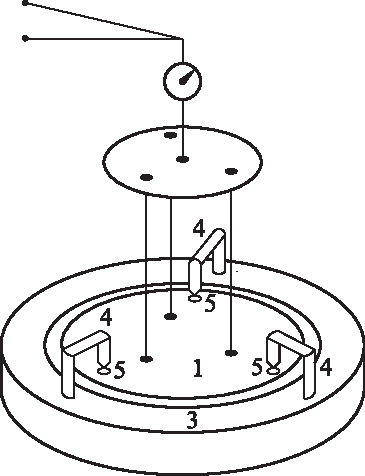
\includegraphics[width=0.38\textwidth]{1_2_2}
	\caption{Конструкция крепления подвижной пластины конденсатора}
	\labfigmark{voltmeter-capacitor}
\end{wrapfigure}

Измерения проводятся в условиях равновесия электрических и механических сил. Как следует из формулы (\r{2}),
электрические силы быстро возрастают с уменьшением зазора между пластинами. С другой стороны, механические силы,
обеспечивающие равновесие аналитических весов, возрастают при наклонах коромысла крайне медленно. В условиях нашего
опыта равновесие весов при равенстве электрических и механических сил оказывается поэтому неустойчивым.

При настройке прибора на левую чашку весов кладётся некоторый перегрузок. При этом положение весов фиксируется тремя
контактными винтами 4, расположенными в~вершинах равностороннего треугольника (\labfigref{voltmeter-experiment} и \r{2}). Винты упираются в
контактные площадки 5, установленные на верхней плоскости подвижной пластины. Напряжение на пластинах регулируется с
помощью реостата $R$ выпрямителя. Электрические силы, действующие на пластину 1, возрастают по мере увеличения
потенциала неподвижной пластины. В тот момент, когда эти силы сравниваются с~весом перегрузка, коромысло теряет
устойчивость и подвижная пластина <<прилипает>> к неподвижной. Этот момент фиксируется по движению стрелки весов.

\begin{lab:task}
	
	В работе предлагается исследовать связь между силой  притяжения пластин и разностью потенциалов между ними для
	определения электрической постоянной $\epsilon_0$ и коэффициента перевода единиц напряжения из системы СГС в систему СИ.
	
	\warning{Регулировка измерительного конденсатора требует определённых навыков и может производиться \important{только
	лаборантом или механиком}. Студент проверяет регулировку пластин визуально, не меняя их настройку самостоятельно.}
	
	\begin{enumerate}
		\item Перед началом работы рассчитайте по формуле (\r{2}) максимально допустимую нагрузку, исходя из предела измерений
		электростатического вольтметра. Расстояние между пластинами~$d$ и площадь пластин~$S$ указаны на установке.
		
		\item Соберите схему согласно Рис.~\ref{fig:voltmeter-experiment}.
		
		По уровню, расположенному на основании весов, проверьте, занимает ли платформа весов горизонтальное положение. При этом
		подвижная пластина измерительного конденсатора должна располагаться в~центре охранного кольца, не касаясь его. При
		обнаружении неисправностей обратитесь к лаборанту.
		
		Проверьте регулировку положения равновесия коромысла ненагруженных весов. Для этого следует отключить пластины
		конденсатора от выпрямителя и соединить их друг с другом (ключ К на Рис.~\ref{fig:voltmeter-experiment} переводится в нижнее положение). Осторожно,
		чтобы не сбить опорные призмы коромысла, освободите весы от арретира. В положении равновесия при закороченных пластинах
		упорные штифты должны быть близки к контактным пластинам и должны касаться их при незначительных ($\sim 10$~мг)
		перегрузках на левой чашке весов.
		
		При необходимости проведите регулировку положения коромысла весов. Для этого снова арретируйте весы и, перемещая
		тарировочные гайки, расположенные на концах коромысла, добейтесь того, чтобы стрелка весов оказалась на нулевом делении
		шкалы. Поворот гаек и изменение груза на чашке весов \important{всегда производятся при арретированных весах}, а проверка
		положения коромысла~--- когда весы сняты с арретира. Для изменения груза открываются боковые дверцы весов (фронтальная
		дверца открывается только на время ремонта).
		
		\item Исследуйте зависимость силы притяжения пластин от напряжения на конденсаторе. Для измерения напряжения применяется
		электростатический вольтметр (вольтметр, вмонтированный в выпрямитель, для измерений не используется).
		
		Переведите ключ К в положение измерения. Положите на левую чашку весов груз, равный примерно 0,1 от максимально
		допустимого. При этом подвижная пластина должна прижаться к упорным штифтам. Подберите напряжение, приводящее к потере
		устойчивости весов. Оно соответствует моменту начала движения стрелки весов.
		
		Рекомендуется уточнить это напряжение 2--3 раза, каждый раз всё медленнее поворачивая ручку реостата $R$. Перед каждым
		измерением напряжения следует закорачивать пластины конденсатора ключом К, чтобы снять с пластин остаточный заряд.
		
		Проведите такие измерения не менее чем в десяти точках, равномерно расположенных в рабочем диапазоне нагрузок.
		
		\item Сразу после измерений изобразите результаты на графике в координатах $F$, $U^2$. Если полученные точки в пределах
		ошибок опыта ложатся на прямую линию, эксперимент можно закончить. Если прямой линии не получилось, следует найти и
		устранить ошибку.
		
		\item По наклону прямой $F=f(U^2)$  рассчитайте значение электрической постоянной $\epsilon_0$.
		
		\item Используйте результаты измерений для определения коэффициента перевода единиц напряжения из системы СГС в систему СИ.
		Напряжение в единицах СГС может быть вычислено по формуле (\r{4}), а показания электростатического вольтметра позволяют
		определить это напряжение в вольтах. Изобразите полученные результаты на графике в координатах $U$~(в~СГС)$=f(U,~В)$ и по
		наклону прямой, проведённой через экспериментальные точки, определите коэффициент пересчёта напряжений.

	\end{enumerate}

\end{lab:task}

\begin{lab:questions}
	\item Оцените ошибку, возникающую вследствие того, что равновесие весов устанавливалось при наличии небольшого зазора между
	штифтами и контактными пластинами, а измерения производятся при отсутствии этого зазора.
	
	\item Покажите, что электростатический вольтметр пригоден для измерения как постоянного, так и переменного напряжения.
	
	\item Покажите, что измерения на переменном токе определяют именно эффективное значение его напряжения.
	
	\item Чем определяется интервал частот, в котором можно измерять переменные напряжения с помощью электростатического
	вольтметра?
\end{lab:questions}

\begin{lab:literature}
	\item {\em Сивухин Д.В.} Общий курс физики. Т.~III. Электричество --- М.: Наука, 1983, \S~125.
	
	\item {\em Калашников С.Г.} Электричество.~--- М.: Наука, 1977, \S\S~5, 6, 26.
	
	%\item {\em Кингсеп А.С., Локшин Г.Р., Ольхов О.А.} Основы физики. Т.~1. Ч.~III. Электричество и магнетизм.~--- М.:
	%Физматлит, 2001.
\end{lab:literature}



% ?
%\input {1_3}
